% CVPR 2026 submission -- Oriented DensePose
% Build:  pdflatex main ; bibtex main ; pdflatex main ; pdflatex main

\documentclass[10pt,twocolumn,letterpaper]{article}

%%%%%%%%% PAPER TYPE
% \usepackage{cvpr}              % CAMERA-READY
\usepackage[review]{cvpr}        % REVIEW version
% \usepackage[pagenumbers]{cvpr} % arXiv version

%% This file contains a number of tweaks that are typically applied to the main document.
%% They are not enabled by default, but can be enabled by uncommenting the relevant lines.


%%
%% Official support for 2-column teaser figure
%%
\usepackage{cuted} %< for strip environment

%%
%% For auto-referencing of figures (see fig/teaser.tex and \label{} therein) 
%%
\usepackage{currfile} %< for \currfilebase macro

%%
%% caption and (global) spacing overrides
%%
\usepackage{caption} %< for "\captionof" commands (teaser)
\setlength{\abovecaptionskip}{.4em}
\setlength{\belowcaptionskip}{0pt}

%%
%% Inline annotations; for predefined colors, refer to "dvipsnames" in the xcolor package:
%% https://tinyurl.com/overleaf-colors
%%
\newcommand{\red}[1]{{\color{red}#1}}
\newcommand{\todo}[1]{{\color{red}#1}}
\newcommand{\TODO}[1]{\textbf{\color{red}[TODO: #1]}}
%%
%% Disable for camera ready / submission by uncommenting these lines:
%%
\renewcommand{\TODO}[1]{}
\renewcommand{\todo}[1]{#1}

%%
%% Work harder in optimizing text layout. Typically shrinks text by 1/6 of page, enable
%% it at the very end of the writing process, when you are just above the page limit.
%%
\usepackage{microtype}

%%
%% Fine-tune paragraph spacing.
%%
% \renewcommand{\paragraph}[1]{\vspace{.5em}\noindent\textbf{#1.}}

%%
%% Globally adjusts space between figure and caption.
%%
% \setlength{\abovecaptionskip}{.5em}

%%
%% Allows "the use of \paper to refer to the project name"
%% with automatic management of space at the end of the word.
%%
% \usepackage{xspace}
% \newcommand{\paper}{ProjectName\xspace}

%%
%% Commonly used math definitions.
%%
% \DeclareMathOperator*{\argmin}{arg\,min}
% \DeclareMathOperator*{\argmax}{arg\,max}

%%
%% Tighten underline.
%%
% \usepackage{soul}
% \setuldepth{foobar}

%%
%% Reconfigure paragraph (tweaks spacing)
%%

%% Float packing (spacing only; no change to margins or fonts)
\setlength{\textfloatsep}{8pt plus 2pt minus 2pt}
\setlength{\floatsep}{6pt plus 2pt minus 2pt}
\setlength{\intextsep}{6pt plus 2pt minus 2pt}
\setlength{\dblfloatsep}{6pt plus 2pt minus 2pt}
\setlength{\dbltextfloatsep}{8pt plus 2pt minus 2pt}
\renewcommand{\topfraction}{0.92}
\renewcommand{\bottomfraction}{0.7}
\renewcommand{\textfraction}{0.06}
\renewcommand{\floatpagefraction}{0.85}
\renewcommand{\dbltopfraction}{0.92}
\renewcommand{\dblfloatpagefraction}{0.85}
\setcounter{topnumber}{3}
\setcounter{bottomnumber}{2}
\setcounter{totalnumber}{4}
\setcounter{dbltopnumber}{2}


\definecolor{cvprblue}{rgb}{0.21,0.49,0.74}
\usepackage[pagebackref,breaklinks,colorlinks,allcolors=cvprblue]{hyperref}

%%%%%%%%% PAPER ID
\def\paperID{*****}
\def\confName{CVPR}
\def\confYear{2026}

%%%%%%%%% TITLE
\title{Oriented DensePose: From Surface Points to Surface Frames}

%%%%%%%%% AUTHORS (anonymous for review)
\author{Anonymous \confName~submission\\
Paper ID \paperID
}

\begin{document}
\maketitle

\begin{abstract}
DensePose tells a downstream model \emph{where} a pixel lies on the body, not
\emph{how the surface is turned} there. We add the missing rotational degrees of
freedom: a DINOv3+DPT network predicting, per pixel and in one pass, the usual part
index and chart coordinates \emph{and} a full $SO(3)$ surface frame --- to our
knowledge the first orientation output for DensePose. Anchored to the body template
rather than the chart, the frame is continuous across chart seams, and composing it
forward transports any template-attached direction into the image: camera-space
normals, hair and weave tangents, and the twist about the normal that a normal map
cannot carry. The model reaches $0.741$ geodesic-point-similarity (GPS) AP on
DensePose-COCO minival under a ground-truth-box protocol, above every model in our own
lineage --- though we re-score no published system under this harness, and the oriented
output costs $2.1$ AP points at matched training step before the recipe recovers them.
Retraining a CVPR'25 pose-guided generator with our correspondence model as the one
changed input improves paired LPIPS by $0.0116$, better on $68.7\%$ of $8{,}512$ pairs
and of the same order as the largest published step on that benchmark; FID does not
move. Predicting a frame correctly is also what forced us to repair the correspondence:
the official DP24 charts are non-injective on roughly half the hand and foot surface at
a median $3$D collision of $60$--$67$\,mm, which a sheet split removes; we supervise
correspondence in metres through a differentiable chart-to-template operator ($-46\%$
hand and foot surface error against a matched control); and we add occlusion data under
a sequence-level holdout ($14.80^\circ\!\rightarrow\!6.89^\circ$ frame error there).

\end{abstract}

\section{Introduction}
\label{sec:intro}

\begin{figure*}[!tb]
\centering
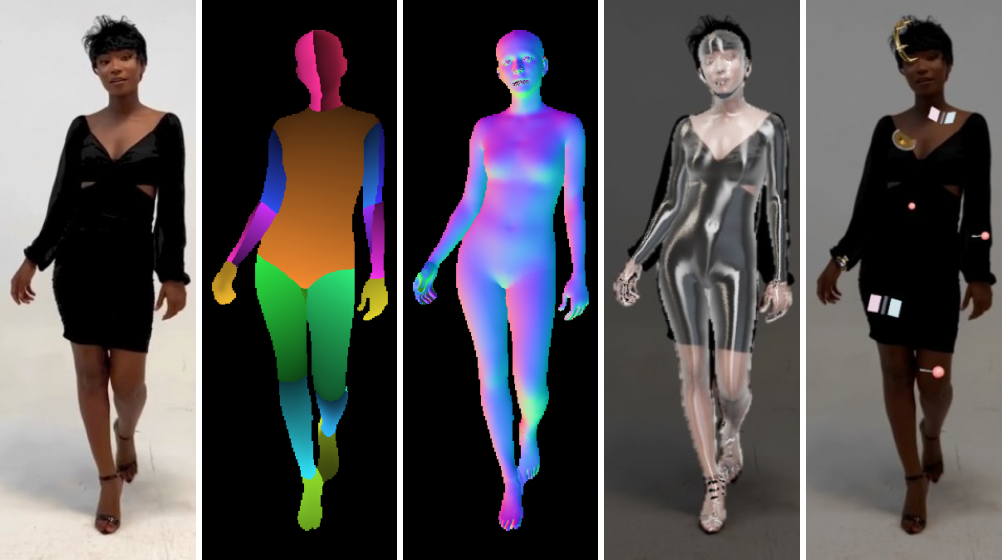
\includegraphics[width=0.42\linewidth]{figs/fig_teaser.png}
\caption{\textbf{Oriented DensePose.} Per pixel, in one pass: the correspondence $(I,U,V)$
\emph{and} a surface frame $\hat R\in SO(3)$; then $\hat R\,\mathbf{n}_{T}$ as a camera-space normal
map, smooth across part seams; satin whose highlight \emph{direction} is set by the twist of
$\hat R$ about the normal; and objects attached at clicked pixels and oriented by $\hat R$.}
\label{fig:teaser}
\end{figure*}

DensePose~\cite{guler2018densepose} defined a task a large family of human-centric systems now
takes for granted: for every foreground pixel of a person, name the point of a canonical body
surface that projects there. Its output --- a part index and two chart coordinates, $(I,U,V)$ ---
became an unusually durable interface, consumed by pose-guided synthesis, garment transfer, avatar
reconstruction and video
re-animation~\cite{neverova2018dpt,pidm2023,cfld2024,fpdm2024,mcld2025,leffa2025}. Those consumers
have been rebuilt more than once, and DensePose accuracy work did
continue~\cite{yang2019parsingrcnn,neverova2019slim,neverova2020cse} --- but the predictor they
import is, overwhelmingly, the detectron2 ResNet-101 released in 2019~\cite{wu2019detectron2}. We
revisit the producer, asking whether its \emph{output} is rich enough, and find that answering that
forces a second question, whether its \emph{supervision} is correct.

\paragraph{The output.}
A correspondence says where a pixel lies, not how the surface is turned there: a template point has
two degrees of freedom, and a frame there adds the three rotational ones. We predict per pixel a
rotation $R\in SO(3)$ carrying the template's own surface frame at the corresponding point into the
camera frame, so $R\,\mathbf{n}_{T}$ is the camera-space normal, $R\,\mathbf{t}$ transports any
template tangent --- the direction a hair or woven fibre runs --- and $R$ in full supplies the
twist about the normal, which a normal map cannot express but which separates a satin highlight or
an object glued to a moving limb from a plausible-looking smear (\cref{fig:teaser}). Anchored to
the template rather than the chart, the frame is \emph{chart-independent}: continuous across seams
and unchanged by a re-cut of the atlas.

\paragraph{The supervision.}
Predicting a frame is what forced us to fix the correspondence, because three defects a chart-space
regression tolerates become visible once the target is geometric. \emph{(i) The charts fold}: a
hand is one part and its chart a planar projection, so palm folds onto back, and roughly $49\%$ of
hand and $53\%$ of foot surface carries a label claimed by more than one surface point at a median
collision of $60$--$67$\,mm --- the ground truth asks for one answer where there are two skin points
$6$\,cm apart, and a sheet split removes it (\cref{sec:charts}). \emph{(ii) A chart-space loss is
blind to metric error}, since charts are renormalised by their own extent and $UV$ is discontinuous
at seams where the surface is not; we supervise in template space through a differentiable
$(i,u,v)\!\rightarrow\!XYZ$ operator (\cref{sec:csc}). \emph{(iii) Occlusion is missing, and labels
must never be resampled}: we train on multi-person contact data under a sequence-level holdout,
mask unlearnable geometry, and rasterise ground truth once into a fixed canvas, warping the
\emph{prediction} into it, because resampling a rotation field averages the frames of two different
surfaces at every occlusion boundary (\cref{sec:data}).

\paragraph{Results, and what they are not.}
Our network reaches $0.741$ GPS AP on DensePose-COCO minival under a ground-truth-box protocol
(\cref{tab:coco}), above every model in our own lineage, while emitting the frame field. No
published DensePose model has been re-scored under this harness, so we claim no state of the art;
the margin over our best $IUV$-only checkpoint is $0.3$ AP points and that checkpoint was chosen by
a sweep on the same minival, so we read the result as \emph{parity plus an extra output} rather
than a win, and orientation is not free at matched step either --- it costs $2.1$ AP points there
(\cref{tab:recipe}), which the final recipe more than recovers. The frame field reaches
$6.77^\circ$ end-to-end geodesic error on held-out synthetic data, against no external baseline,
because none exists and we did not build one. Downstream, a test-time swap into a pretrained
generator proves nothing, since the host is fit to its own conditioner's error distribution; we
therefore retrain MCLD (CVPR'25)~\cite{mcld2025} twice with the authors' unmodified code, same
images, seed and schedule, changing only the DensePose model. Ours improves paired LPIPS by
$0.0116$ (better on $68.7\%$ of $8{,}512$ pairs) together with SSIM and PSNR, of the same order as
the largest published LPIPS step on this benchmark ($0.0037$, which \emph{lost} SSIM, PSNR and
FID), while FID does not move --- the correct signature, since correspondences buy spatial fidelity
and FID measures a distributional realism set by the fixed diffusion prior. That host consumes only
$IUV$, so it measures the correspondence half of our output.

\paragraph{Contributions.}
(1) \textbf{Oriented DensePose}, the first per-pixel $SO(3)$ output for DensePose, at a measured
cost of $2.1$ AP points at matched step which the final recipe recovers. (2) \textbf{A fold-free
re-flattening of the hand and foot charts} ($49\%/53\%\!\rightarrow\!0.0\%/0.7\%$), correcting a
label defect inherited since 2019 with $20$ of $24$ charts bit-identical; the head charts are
\emph{not} fixed, only masked. (3) \textbf{A canonical-surface-coordinate loss} supervising
correspondence in metres, with an exact rather than heuristic validity test. (4) \textbf{Occlusion
supervision under a sequence-level holdout} and a hidden-geometry mask --- the first ablated, the
second documented but not. (5) \textbf{A recipe diagnosis}: the base learning rate and
over-training on synthetic data, not the rotation task, explain our lineage's real-domain deficit.
(6) \textbf{A controlled downstream measurement} of what the correspondence model is worth to a
generator, with the host retrained rather than swapped at inference.

\section{Related Work}
\label{sec:related}

\paragraph{Dense human correspondence and its supervision.}
DensePose~\cite{guler2018densepose} maps foreground pixels to points on the
SMPL~\cite{loper2015smpl} surface via a part index and two chart coordinates, and introduced the
DensePose-COCO benchmark and the geodesic point similarity (GPS) we use; its $24$ planar PCA charts
and the ResNet-101 predictor released with detectron2~\cite{wu2019detectron2} have been inherited
essentially unchanged, though accuracy work
continued~\cite{yang2019parsingrcnn,neverova2019slim,neverova2020cse,neverova2021ucm,shapovalov2021densepose3d,ianina2022bodymap,pozdeev2025densemarks,tan2021humangps}.
All predict a surface \emph{point}; none a surface \emph{frame}. We keep charts, because they are
the interface the ecosystem consumes, repair a defect in their labels, and recover the metric
consistency that motivated CSE~\cite{neverova2020cse} and continuous UV maps~\cite{zeng2020decomr}
through the \emph{loss} rather than the representation; regressing a canonical surface coordinate
in metres is standard in dense object
pose~\cite{wang2019nocs,park2019pix2pose,hodan2020epos,haugaard2022surfemb}, and our contribution
there is not the idea but its exact validity test on a folded atlas. Synthetic
corpora~\cite{varol2017surreal,patel2021agora,black2023bedlam,tesch2025bedlam2} give every pixel an
exact face index and barycentric weights, hence \emph{any} per-pixel quantity derivable from the
mesh --- a surface frame included, which is what makes an orientation target available at all; for
occlusion and body-to-body
contact~\cite{fieraru2020chi3d,yin2023hi4d,khirodkar2024harmony4d,xu2024interx} we train on MAMMA's
synthetic corpus~\cite{cuevas2025mamma} under a sequence-level holdout.

\paragraph{Orientation: normals, rotations, frame fields.}
Monocular networks have long emitted per-pixel directions~\cite{eigen2015multiscale} and dedicated
normals~\cite{bae2021nll,bae2024dsine}, including for clothed
humans~\cite{saito2020pifuhd,xiu2022icon} and as one head of a human-centric foundation
model~\cite{khirodkar2024sapiens}; our multi-scale gradient term follows the scale-invariant depth
literature~\cite{eigen2015multiscale,li2018megadepth,ranftl2020midas}, applied to correspondence. A
normal leaves the rotation about itself undetermined, and that twist decides how an anisotropic
highlight, a hair strand or an attached object sits on the body. Frame fields are mature in geometry
processing~\cite{ray2008nsym,bommes2009miq,knoppel2013direction,vaxman2016directional}, where the
field is optimised on a mesh already given, and have been predicted from images as 2D $4$-RoSy
fields for building extraction~\cite{girard2021framefield}; here the predicted object is a full
element of $SO(3)$ anchored to a body template. We use the continuous 6D
parameterisation~\cite{zhou2019continuity} with a chordal objective, a monotone function of the
geodesic angle~\cite{huynh2009metrics}; SVD orthogonalisation~\cite{levinson2020svd} is the
standard alternative and modelling the full $SO(3)$ distribution~\cite{murphy2021ipdf} the natural
treatment of the ambiguity on near-cylindrical limbs. Our target is the local as-rigid-as-possible
rotation~\cite{sorkine2007arap} of the one-ring, by Kabsch~\cite{kabsch1976} with a normal pin. We
are not aware of prior work predicting a per-pixel $SO(3)$ element on the human body from an image.

\paragraph{Consumers of DensePose.}
$IUV$ maps condition pose-guided
synthesis~\cite{neverova2018dpt,ren2022nted,zhou2022casd,pidm2023,shen2024pcdm,cfld2024,pham2024xmdpt,mcld2025,fpdm2024,leffa2025},
try-on~\cite{choi2021vitonhd,kim2024stableviton,choi2024idmvton},
animation~\cite{xu2024magicanimate,zhu2024champ} and mesh and avatar
recovery~\cite{guler2019holopose,xu2019denserac,zeng2020decomr,shysheya2019tna}. Throughout the
correspondence is a \emph{fixed input}: the predictor is imported and frozen and the contribution
is architectural, so progress is measured by changing the consumer --- the largest published LPIPS
step on DeepFashion pose transfer, MCLD~\cite{mcld2025} to FPDM~\cite{fpdm2024}, is $0.0037$,
obtained while losing SSIM, PSNR and FID. That some systems render SMPL normals as extra
conditioning~\cite{zhu2024champ} shows the demand for surface geometry; they obtain it by fitting a
body model, the most obvious baseline for our frame field and one we did not run. What the
correspondence \emph{input} is worth has, to our knowledge, never been measured, because measuring
it means retraining the consumer; \cref{sec:exp_down} does that.

\section{Method}
\label{sec:method}

\begin{figure*}[!tb]
\centering
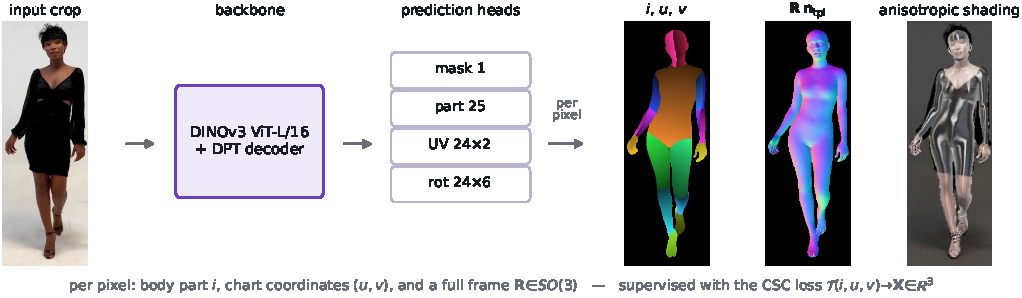
\includegraphics[width=0.58\linewidth]{figs/fig_method.pdf}
\caption{\textbf{Pipeline.} A person crop is encoded by DINOv3 ViT-L/16 and a DPT decoder into
four heads --- body mask, $24$-way part, $24{\times}2$ chart coordinates, $24{\times}6$ rotation ---
read out per pixel as $(\hat\imath,\hat u,\hat v,\hat R)$; correspondence is supervised in metric
template space through the operator $\Phi$ of \cref{sec:csc} and rotation by a chordal loss against
the template's own surface frame.}
\label{fig:method}
\end{figure*}

\subsection{From surface points to surface frames}
\label{sec:task}

Let $T$ be a fixed template (neutral SMPL-X~\cite{pavlakos2019smplx}) partitioned into the $24$
DensePose parts, each with a chart $\mathcal{C}_i\subset[0,1]^2$. The classical task predicts at
every pixel $x$ a body flag $\hat m$, a part $\hat\imath$ and chart coordinates $(\hat u,\hat v)$
--- together a template point $\pi(x)$. We add $\hat R(x)\in SO(3)$, the rotation carrying the
template's \emph{own} surface frame at $\pi(x)$ into the camera-space frame of the posed surface,
so that $\hat R\,\mathbf{n}_T(\pi(x))=\mathbf{n}_{\mathrm{cam}}(x)$ and
$\hat R\,\mathbf{t}=\mathbf{t}_{\mathrm{cam}}(x)$ for \emph{any} template-attached $\mathbf{t}$.
Anchoring to the template rather than the chart matters: a chart-induced tangent frame would flip
at seams, be undefined where the chart degenerates, and change meaning under a re-cut, including
our own. It remains a gauge choice --- fixed by the template's tessellation through
\cref{eq:kabsch} --- but it makes the target \emph{chart-independent} and continuous across part
boundaries, so its ground truth is a per-vertex field. Since $SO(3)$ has no continuous global
three-parameter chart the net emits $g\in\mathbb{R}^6$~\cite{zhou2019continuity}, mapped to
$\psi(g)\in SO(3)$ by Gram--Schmidt.

The backbone is DINOv3 ViT-L/16~\cite{dinov3}: tokens after blocks $\{4,11,17,23\}$ are projected
to $d{=}256$, resampled to $\{4,2,1,0.5\}\times$ the token grid and fused by four DPT
blocks~\cite{ranftl2021dpt}, only the patch embedding frozen ($302$M of $303$M parameters train).
Four heads predict a body mask (BCE over \emph{all} pixels), $24$ parts (cross-entropy on
foreground), $24{\times}2$ chart coordinates (smooth-$L_1$ on the ground-truth part's channels) and
$24{\times}6$ rotation. The $25$-way readout is \emph{factorised} into a binary body head and a
$24$-way part head with no background class, so the part head cannot resolve an ambiguous seam by
predicting background. A per-part rather than shared rotation head buys $0.53^\circ$ of geodesic
error at matched step with synthetic part accuracy and UV error unchanged, but costs $1.8$ COCO AP
points (\cref{tab:recipe}); we ship it and the final recipe recovers the AP. At test time we take
$\hat\imath=\arg\max_i\hat s_i$ where $\hat m>0$ and gather $(\hat u,\hat v)$ and $\hat R$ from
that part, so every COCO number and every end-to-end geodesic error includes part-classification
error; metrics gathered by the ground-truth part are labelled \emph{oracle}. Wherever a per-part
volume is resampled --- as in COCO scoring, on the box expanded by $1.2\times$ --- we resize the
\emph{volume} and gather afterwards, since resizing the gathered map blends adjacent parts.

\subsection{Rotation supervision}
\label{sec:rotsup}

The target $R_v$ is the local as-rigid-as-possible rotation~\cite{sorkine2007arap} of the one-ring
$\mathcal{N}(v)$ between template vertices $\bar V$ and camera-space vertices $V$: a Kabsch
problem~\cite{kabsch1976} with a normal pin, solved by SVD $H_v=U\Sigma W^{\!\top}$,
$R_v=W\,\mathrm{diag}(1,1,\det(WU^{\!\top}))\,U^{\!\top}$, where
\begin{equation}
  H_v \!=\!\!\! \sum_{j \in \mathcal{N}(v)} \!\!\! (\bar V_j \!-\! \bar V_v)(V_j \!-\! V_v)^{\!\top}
      \!\!+ \lambda \Big(\!\!\!\sum_{j \in \mathcal{N}(v)}\!\!\! \lVert \bar V_j \!-\! \bar V_v \rVert^2 \Big)
        \bar n_v n_v^{\!\top}\!,
  \label{eq:kabsch}
\end{equation}
$\lambda{=}25$ and $\bar n_v,n_v$ the area-weighted unit vertex normals. Without the pin this is a
pure edge fit whose third axis is whatever the one-ring implies; the pin pulls it towards the
surface normal, which is what makes the transport identity useful. The pin is \emph{soft}, so that
identity holds only approximately, and we measured neither the residual angle nor the sensitivity
to $\lambda$. The per-pixel label is the barycentric blend of the rasterised face's three vertex
$6$D vectors through $\psi$ --- formally the operation \cref{sec:data} argues against, but at the
scale of one triangle, where the three frames are near-parallel; we rely on that and do not measure
it. Labels come from the \emph{body} surface, so on clothed regions the frame is that of the body
beneath the garment. On the foreground $M$, gathering the ground-truth part's six channels, the
loss is chordal, $|M|^{-1}\sum_x\lVert\psi(\hat
g_{i_{\mathrm{gt}}(x)}(x))-R_{\mathrm{gt}}(x)\rVert_F^2$: since $\lVert
R_1-R_2\rVert_F^2=4(1-\cos\theta)$ it is a monotone surrogate for the geodesic angle $\theta$ that
keeps $\arccos$ out of the graph~\cite{hartley2013rotation}.

\subsection{Fold-free charts}
\label{sec:charts}

The official atlas builds each chart as a planar PCA projection of its part. For the $18$
half-cylinder parts this is injective; for hands and feet it is not, because a hand is \emph{one}
part containing palm, back and fingers, and sampling surface points to count how many of the part's
triangles claim each $(u,v)$ shows roughly $49\%$ of hand and $53\%$ of foot surface non-injective,
at a median $3$D distance of $60$--$67$\,mm between claimants (supp.). We re-flatten those four
parts by splitting each into two \emph{sheets} on the sign of $\langle n_f,n_i\rangle$ --- face
normal against chart-plane normal, i.e.\ palm/back and top/sole --- keeping the original PCA
projection, renormalising within each sheet and packing the sheets into halves of the unit square
with a gutter no bilinear stencil can span; within a sheet the surface is a height field over the
chart plane, so the projection that folded becomes single-valued. This is exact only away from the
rim, where $\langle n_f,n_i\rangle\!\approx\!0$ makes the assignment arbitrary: residual overlap is
$0.0\%$ (hands) and $0.7\%$ (feet), and the split adds a rim seam and a per-sheet scale, neither
measured. The head is left unchanged, its residual being hidden geometry \emph{inside} the part and
identical (${\approx}0.6\%$) in \textsc{v1} and \textsc{v2}, so the atlas is fold-free on hands and
feet and the head is masked, not fixed. Nothing in the model changes: the loader derives
ground-truth UV from the face-UV asset on the fly, so swapping it needs \emph{no} re-sharding
($3.7$\,TB untouched) and $20$ of $24$ charts stay bit-identical. COCO annotations are \textsc{v1},
so a \textsc{v2} model is scored through an exact texel-wise remap, and joint COCO fine-tuning
\emph{skips} the sparse UV term on parts $3$--$6$ while keeping their part cross-entropy, because
COCO's UV labels there are \textsc{v1} and \textsc{v1} is fold-ambiguous there anyway.

\subsection{Canonical surface coordinates}
\label{sec:csc}

Three properties of the atlas make a smooth-$L_1$ on $(u,v)$ a poor objective: charts are
renormalised by their own PCA span and spans differ $8\times$; $(u,v)$ jumps at seams where the
surface does not, and $6.1\%$ of template vertices touch more than one chart; and a pointwise loss
constrains the value of the correspondence map but not its spatial derivative, the local geometry
any consumer of a frame reads --- we offer this third one as motivation, not measurement. We
therefore bake, per part, a $512^2$ texture $T_i$ of template XYZ over that part's chart by
barycentric rasterisation and read it as $\Phi(i,u,v)=\mathrm{bilinear}(T_i,(u,v))$ with one 3D
\texttt{grid\_sample} whose part axis lands on slice centres, so part selection is exact and $\Phi$
is differentiable in $(u,v)$ with an exact analytic Jacobian. Against exact barycentric XYZ on
$200$k surface points, on the $74.5\%$ an ambiguity mask admits, median error is below $0.001$\,mm
and p99 is $0.335$\,mm, but the maximum is $63$\,mm on sliver triangles, so our own $\max<1$\,mm
criterion fails: $\Phi$ is exact for the overwhelming majority of the surface and \emph{not}
uniformly so, and we accept that tail rather than claim it away, because the losses are $L_1$
averages over millions of pixels (supp.). With $\hat X(x)=\Phi(i(x),\hat u_{i(x)}(x),\hat
v_{i(x)}(x))$,
\begin{align}
  \mathcal{L}_{\mathrm{xyz}}
    &= \tfrac{1}{3|M'|} \! \sum_{x \in M'} \! \big\lVert \hat X(x) - X_{\mathrm{gt}}(x) \big\rVert_1
    \;\text{[m]}, \label{eq:lxyz}\\
  \mathcal{L}_{\mathrm{grad}}
   &= \tfrac{1}{N} \sum_{s,d} \tfrac{1}{3|E_d^{(s)}|} \!\! \sum_{x \in E_d^{(s)}} \!\!
     \big\lVert \kappa_c(\Delta_d \hat X^{(s)}) - \kappa_c(\Delta_d X^{(s)}_{\mathrm{gt}}) \big\rVert_1 ,
  \label{eq:lgrad}
\end{align}
the second multi-scale gradient
matching~\cite{eigen2015multiscale,li2018megadepth,ranftl2020midas} on correspondences rather than
depth, over $S{=}4$ scales and axes $d\in\{u,v\}$, with $E_d^{(s)}$ the edges \emph{both} of whose
endpoints are valid and $\kappa_c$ clipping each coordinate to $\pm c{=}0.20$\,m/px. Both sides are
clipped, so \cref{eq:lgrad} is deliberately blind to steps larger than $c$, keeping ${\sim}0.5$\,m
self-occlusion jumps from dominating a term meant to shape smooth structure; at $c{=}0.05$ it goes
blind to the blur it exists to remove. With $M$ the foreground minus hidden faces we keep only
pixels where the chart reproduces the pixel's own known $3$D point,
\begin{equation}
  M' \!=\! M \cap \Big\{ x : \big\lVert \Phi\big(i_{\mathrm{gt}},u_{\mathrm{gt}},v_{\mathrm{gt}}\big)(x)
       - X_{\mathrm{gt}}(x) \big\rVert_2 < \tau \Big\},\; \tau{=}5\,\mathrm{mm}.
  \label{eq:valid}
\end{equation}
The test is exact rather than heuristic because $i_{\mathrm{gt}}$, $(u,v)_{\mathrm{gt}}$ and
$X_{\mathrm{gt}}$ derive from the \emph{same} rasterised face and barycentrics, so every pixel
knows its own true template point and the loss can simply ask the chart to reproduce it; where the
chart folds or covers hidden geometry it fails and the pixel drops, so the fold mask falls out of
the construction rather than being hand-tuned. We never logged $|M'|/|M|$, so the fraction of
foreground receiving metric supervision is unmeasured; $\hat u$ is gathered by the ground-truth
part, one of three variants (\cref{sec:exp_csc}). The objective adds $\mathcal{L}_{\mathrm{mask}}$,
$\mathcal{L}_{\mathrm{part}}$, $\mathcal{L}_{\mathrm{uv}}$ and $\mathcal{L}_{\mathrm{rot}}$ at
weight $1$ to $\mathcal{L}_{\mathrm{xyz}}$ at $2$ and $\mathcal{L}_{\mathrm{grad}}$ at $5$.

\subsection{Training data and label integrity}
\label{sec:data}

We train on BEDLAM2~\cite{tesch2025bedlam2} for clean single-person coverage and
MAMMA-syn~\cite{cuevas2025mamma} for multi-person contact, mixed ${\approx}50/50$. Because MAMMA is
our evidence that occlusion supervision transfers, we hold out \emph{sequences}, not frames:
$\mathrm{md5}(\text{seq})\bmod50=0$ selects $29$ of $2211$ sequences ($59$ of $5417$ shards) across
all four sub-datasets, and shard names embed sequence ids, so the exclusion is exact.

The faithful DensePose loss never resamples labels, and with a rotation field the cost of breaking
that rule is measurable: bilinearly resizing a $6$D field \emph{averages the rotations of two
different surfaces} wherever a limb occludes the torso, and Gram--Schmidt of that blend is a frame
belonging to neither --- on MAMMA at $832\!\rightarrow\!384$, $4.4\%$ of labels are wrong by more
than $10^\circ$ and $3.2\%$ by more than $30^\circ$, up to a $180^\circ$ flip, concentrated at
exactly the occlusion boundaries the occlusion data exists to teach. We therefore rasterise ground
truth once into a fixed $512^2$ canvas ($1.2\times$ the tight body box) and never touch it again,
warping the \emph{prediction} into it with one closed-form \texttt{grid\_sample} per head:
\emph{the direction is the argument}, since a network output is a smooth field that warping merely
\emph{evaluates} at the ground truth's pixel centres, whereas the ground truth has true
discontinuities that warping destroys. Because the canvas is fixed-size the loss also stacks, so
every head, including the $144$-channel rotation field, is supervised at full $512^2$; crops stay
concentric with scale jitter $1.25$--$1.4\times$, and horizontal flip is disabled whenever the
rotation head is active, since a mirrored rotation ground truth is not implemented. SMPL-X also
carries geometry never visible yet still winning rasterisation --- eyeballs, mouth cavity, inner
lips and eye sockets, $3870$ of $20\,908$ faces, $0.106\%$ of foreground --- whose labels are coin
flips; the loader fills the part map first and \emph{then} clears the foreground gate there, so
part, UV, rotation and CSC skip those pixels while the body-mask BCE still sees the whole person.
We optimise with AdamW under layer-wise learning-rate decay (LLRD; $26$ groups, embeddings at
$\text{lr}\cdot0.75^{25}$), grad-clip $1.0$, $500$-step warmup, cosine schedule, batch $32$ per GPU
on $4{\times}$GH200, colour jitter the only further augmentation. The base rate is
$3{\times}10^{-4}$; $10^{-3}$ is the synthetic optimum but costs $3.4$ COCO AP points
(\cref{tab:recipe}). Training is two-stage: $120$k steps on the synthetic mix, then a $10$k-step
joint fine-tune (flat $5{\times}10^{-5}$, half the batches from
DensePose-COCO~\cite{guler2018densepose,lin2014coco} under the sparse loss above), saving every
$1$k steps; selection is discussed in \cref{sec:exp_main}.

% Provenance: every number traces to paper/RESULTS.md or the job log in the trailing comment.
\section{Experiments: correspondence}
\label{sec:exp_corr}

\subsection{Protocol}
\label{sec:exp_setup}

On DensePose-COCO we use the official minival annotations and GPS
implementation~\cite{guler2018densepose,wu2019detectron2}, reporting AP over
$\mathrm{OGPS}=0.50\!:\!0.95$. Because this paper studies the correspondence stage in isolation,
our protocol supplies boxes rather than detections: every annotated ground-truth box becomes a
score-1 detection ($2243$ instances, $1508$ images); for the one model we ran under both protocols
they agree closely ($0.633$ vs.\ $0.624$ with Faster R-CNN boxes), and we do not generalise from a
single pair. On $512$ held-out BEDLAM2~\cite{tesch2025bedlam2} instances we report
\emph{geo\_e2e}, the mean geodesic frame error with the rotation channel gathered by the
\emph{predicted} part, so part misclassification is charged as at deployment (the ground-truth
gather, \emph{geo\_oracle}, is optimistic by $0.4$--$0.7^\circ$ and is never a headline), and
\emph{surface error}, the \emph{median} per-pixel template-space distance; that split is defined at
instance level with no documented sequence-level separation rule, unlike the occlusion probe, which
uses $640$ instances from the held-out MAMMA shards of \cref{sec:data}. All rows share the network
and recipe above: \textbf{W-B} trains on BEDLAM2 only, \textbf{W-M} on BEDLAM2$+$MAMMA,
\textbf{W-J} also interleaves COCO through the synthetic stage, \textbf{W-MF} is W-M plus $3$k
steps of the joint COCO fine-tune, and \textbf{F0} is an earlier checkpoint of the same family,
trained before the sequence holdout, used downstream. The CSC arms A/C/D/E are $25$k-step
fine-tunes from an older $120$k checkpoint outside the W-$*$ lineage (internal run names; there is
no B). Two things we do not have and do not substitute for: no training GPU-hours or inference
latency were measured, and \textbf{every number here comes from a single training run}, so we
report no variance and avoid calling any difference ``noise'' or ``free''.
% dpeval/eval_vitl_final.txt: GT-box 0.633 / DETECTOR-v2 0.624.  RESULTS S2b: 7.30 vs 7.95 @120k

\begin{table}[!tb]
\centering\footnotesize\renewcommand{\arraystretch}{0.94}
\setlength{\tabcolsep}{4pt}
\begin{tabular}{@{}lcccc@{}}
\toprule
 & & COCO & BEDLAM & occl.\\
Model & Rot. & AP & geo$^\circ$ & geo$^\circ$ \\
\midrule
\multicolumn{5}{@{}l}{\emph{ours, IUV only}}\\
DINOv3-DPT, synthetic          & --         & 0.633 & --- & ---\\
\emph{\ \ same, detector boxes} & --        & 0.624 & --- & ---\\
\ \ + COCO ft                  & --         & 0.732 & --- & ---\\
\ \ + joint COCO/BEDLAM ft     & --         & 0.738 & --- & ---\\
\midrule
\multicolumn{5}{@{}l}{\emph{ours, with the frame field}}\\
W-B (BEDLAM only)              & \checkmark & 0.613 & 6.98 & 14.80\\
W-M (\,$+$\,MAMMA)             & \checkmark & 0.621 & \textbf{6.86} & \textbf{6.89}\\
W-J (\,$+$\,COCO interleaved)  & \checkmark & ---   & 7.18 & 10.77\\
\textbf{W-MF @3k} (\,$+$\,joint ft) & \checkmark & \textbf{0.741} & --- & 8.24\\
\bottomrule
\end{tabular}
\caption{\textbf{DensePose-COCO GPS AP (ground-truth boxes unless noted), BEDLAM-val and held-out
occlusion error}; one architecture throughout. \textbf{There is no external row}: no published
DensePose model was re-scored under this harness, so we compare only with our own $IUV$-only
checkpoints and claim no state of the art; $0.741$ is the maximum of a checkpoint sweep on this
same minival. W-B vs.\ W-M is matched-recipe, its only training variable contact data; blanks were
not run. F0 predates the holdout, so its $10.62^\circ$ is not a held-out number. Single run per
row.}
\label{tab:coco}
\end{table}

\subsection{Correspondence accuracy}
\label{sec:exp_main}

\cref{tab:coco} gives the headline: \textbf{W-MF} reaches \textbf{0.741 GPS AP}, $0.3$ AP points
above the strongest $IUV$-only checkpoint of the same architecture and $12.0$ above the same recipe
without its COCO fine-tune, while additionally predicting a surface frame at every pixel. Three
qualifications belong here rather than in a rebuttal. \emph{Selection:} the number is the maximum
of a COCO-GPS sweep over second-stage checkpoints, on the set it is reported on
($0.713$/$0.729$/$\mathbf{0.741}$/$0.737$/$0.734$ at $1$/$2$/$3$/$5$/$10$k), so the selection bias
is of the same order as the margin and we read the table as \emph{parity plus an extra output}, not
a correspondence win. \emph{The oriented output is not free at matched step:} \cref{tab:recipe}
charges it $2.1$ AP points --- $0.3$ for a bundle of three simultaneous changes we cannot separate,
$1.8$ for the per-part rotation head, which serves only rotation and which ships. \emph{The
fine-tune dominates every contribution here:} $12.0$ of the AP comes from the short joint COCO
stage, which is not ours, while every component this paper contributes moves single points.
% mf-gate-5702500.out

\begin{table}[!tb]
\centering\footnotesize\renewcommand{\arraystretch}{0.94}
\setlength{\tabcolsep}{5pt}
\begin{tabular}{@{}lcc@{}}
\toprule
Cumulative change & AP & $\Delta$ \\
\midrule
IUV-only, flat backbone LR              & 0.633 & --    \\
+ rotation task, $-$hflip, factorised head & 0.630 & $-0.3$ \\
+ per-part rotation head                & 0.612 & $-1.8$ \\
+ LLRD backbone LR (base $3\!\cdot\!10^{-4}$) & 0.622 & $+1.0$ \\
+ base LR $10^{-3}$ (synthetic optimum) & 0.588 & $-3.4$ \\
+ 58k $\rightarrow$ 120k pure synthetic & 0.578 & $-1.0$ \\
+ MAMMA 50/50                           & 0.565 & $-1.3$ \\
\bottomrule
\end{tabular}
\caption{\textbf{Recipe diagnosis}, not a component ablation; $\Delta$ in AP points. Rows 1--5 are
matched at step 58k; the last two continue the run to 120k and add occlusion data, so they are not
step-matched, and the last is superseded --- at a corrected learning rate occlusion data is worth
$+0.008$ AP, the opposite sign (\cref{tab:coco}). Rows 2--3 are both attributable to the oriented
output and sum to $-2.1$; row 2 bundles three changes and cannot be decomposed. Single run per
row.}
\label{tab:recipe}
\end{table}

Read as a diagnosis, \cref{tab:recipe} says the deficit our oriented lineage showed on COCO was not
the second task: the synthetic-optimal base learning rate costs $3.4$ AP points and prolonged
pure-synthetic training a further $1.0$. Synthetic rotation error meanwhile improves monotonically
down the same ladder under an oracle readout ($9.01^\circ\!\rightarrow\!7.86^\circ$, supp.), so
real AP and synthetic geodesic error \emph{anti-correlate} along the learning-rate axis and
layer-wise decay at base $3\!\cdot\!10^{-4}$ is the only step improving both. We had checked that
decision with the sparse point-accuracy proxy the training loop already computed, and it moved by
$0.6$ points where GPS AP moved by $3.4$: different statistics, so the ratio means nothing, but one
crossed a decision threshold and the other did not. \emph{Gate recipe decisions on GPS, not on a
sparse proxy.}

\subsection{Charts, CSC, occlusion data and staging}
\label{sec:exp_csc}

\begin{table}[!tb]
\centering\scriptsize\renewcommand{\arraystretch}{0.94}
\setlength{\tabcolsep}{4pt}
\begin{tabular}{lcccc}
\toprule
System & AP & surf (mm) & h+f (mm) & geo ($^\circ$) \\
\midrule
baseline (\textsc{v1} charts)      & 0.565 & 12.54 & 92.58$^{*}$ & ---\\
A\; \textsc{v2} charts, no CSC     & 0.552 & 10.52 & 24.81 & 6.88\\
\textbf{C\; + CSC (GT gather)}     & \textbf{0.568} & \textbf{8.18} & 13.47 & \textbf{6.77}\\
D\; + CSC (argmax gather)          & 0.563 & 8.22  & \textbf{13.46} & 6.90\\
E\; + CSC (soft top-3 gather)      & 0.560 & 8.23  & 13.87 & 6.87\\
\bottomrule
\end{tabular}
\caption{\textbf{CSC ablation}, $25$k fine-tuning steps from a common checkpoint. ``surf'' is
\emph{median} template-space surface error on BEDLAM-val, ``h+f'' the same on hands and feet,
``geo'' end-to-end rotation error. $^{*}$The baseline predicts \textsc{v1} coordinates but is
scored against \textsc{v2} ground truth, so \emph{every} column of that row is
convention-mismatched; row A is the comparison point we use. The common checkpoint is the
broken-LR $120$k model of \cref{tab:recipe} (see text).}
\label{tab:csc}
\end{table}

On what the chart repair is worth in AP we cannot isolate it: the one near-matched comparison is
\cref{tab:csc}'s baseline ($0.565$, \textsc{v1}) against row A ($0.552$, \textsc{v2}, same losses),
\emph{negative} by $1.3$ AP points --- but row A carries $25$k additional pure-synthetic steps that
\cref{tab:recipe} shows cost AP on their own, and we did not run the \textsc{v1} control on that
schedule. A different quantity is often confused with it: the same checkpoint scores $0.568$ with
the \textsc{v2}$\to$\textsc{v1} remap and $0.521$ without, so $4.7$ AP points measure the necessity
of the remap, not the benefit of the re-flattening. The chart contribution is thus a correctness
result. Supervising correspondences in metres cuts median surface error from
$10.52$ to $8.18$\,mm ($-22\%$) and hands/feet error from $24.81$ to $13.47$\,mm
($\mathbf{-46\%}$), and halves the seam-break rate --- the fraction of physically continuous part
boundaries across which the predicted canonical map jumps by more than $30$\,mm --- from $3.08\%$
to $1.47\%$. It also acts as a sim2real regulariser, finishing $1.6$ AP points above row A on COCO;
against the checkpoint both were fine-tuned from the same change is $+0.3$, and both belong in the
reader's hands because the control's own deficit is unexplained. The surface-error result does not
depend on that ambiguity and is the one we lead with; its residual is a misclassified pixel reading
a different chart, and rotation error is flat across the ablation ($6.77$--$6.90^\circ$), so the
part head is the remaining lever. The gather variant barely matters --- $\arg\max$ (D) and a
renormalised top-$3$ mixture (E) give $0.563$/$0.560$ AP against C's $0.568$ at identical surface
error --- and we adopt C without claiming a winner. \textbf{One caveat covers the whole ablation}:
its common checkpoint is the broken-learning-rate $120$k model, not the shipped W-M checkpoint, so
the CSC loss ships with no on/off comparison inside the shipped recipe.
% csc-coco-5668430.out; csc-detail-5662139.out

W-B and W-M, finally, share every element of the recipe and differ only in whether multi-person
contact data is in the mixture. On held-out sequences the difference is $14.80^\circ$ against
$6.89^\circ$, and it costs nothing elsewhere ($+0.008$ AP on COCO, $-0.12^\circ$ on clean
synthetic); an earlier version of the comparison at the bad learning rate appeared to show
occlusion data costing $1.3$ AP points, a recipe artifact whose sign the matched comparison
reverses. One caveat is structural: the probe is held-out \emph{MAMMA}, in-domain for W-M and an
entirely unseen synthetic domain for W-B, so the $-7.9^\circ$ measures occlusion supervision
\emph{and} domain match together --- what we defend is the conjunction, that adding this corpus at
fixed recipe transfers to sequences it never saw and costs nothing on the two other axes we
measure. Staging matters as much: interleaving COCO through the synthetic run (W-J) is worse on
held-out occlusion, and the joint stage buys $12.0$ AP points while giving up $1.35^\circ$ there ---
a mechanism we did not isolate. We ship two checkpoints accordingly.

\section{Orientation}
\label{sec:exp_orient}

\begin{figure*}[!tb]\centering
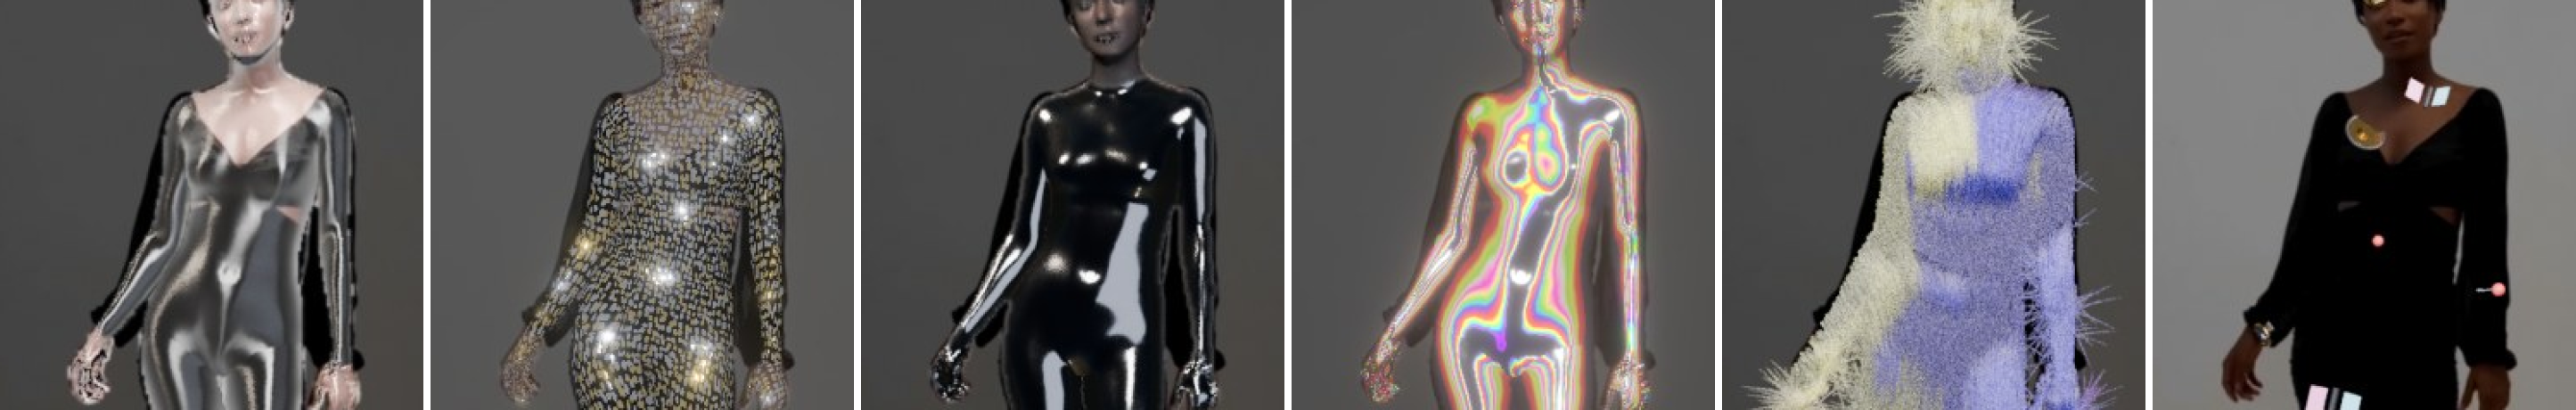
\includegraphics[width=0.94\linewidth]{figs/fig_framefield.png}
\caption{\textbf{The frame field, used forward} on real video: \textbf{(a)} anisotropic satin, a
Kajiya--Kay~\cite{kajiya1989rendering} lobe whose axis is the predicted tangent --- the one effect
a normal map cannot produce; \textbf{(b)} sequins on canonical UV cells, welded to skin not image;
\textbf{(c)} chrome, a readout of the predicted normals; \textbf{(d)} a Stam
grating~\cite{stam1999diffraction} painting twist as colour; \textbf{(e)} Cycles fur along the
unprojected 3D tangent; \textbf{(f)} orientation-locked object attachment. Qualitative: no
orientation ground truth exists for these frames.}
\label{fig:framefield}
\end{figure*}

On BEDLAM-val the shipped models reach $6.77^\circ$ (\texttt{dp\_csc\_C}) and $6.86^\circ$ (W-M)
mean geodesic error under the end-to-end readout, against $6.98^\circ$ for W-B (\cref{tab:coco});
the number is stable across the data and recipe changes of \cref{sec:exp_csc} on this clean split,
and the entire gap opened by occlusion data appears not here but on held-out interaction sequences
($14.80^\circ\!\rightarrow\!6.89^\circ$). What the field buys is qualitative
(\cref{fig:framefield}): each render is a \emph{pullback} of the prediction, so nothing inverts it,
tracks a point, fits a mesh or filters temporally.

\paragraph{We have no baseline for this number, and that is the main weakness of the orientation
result.} $6.77^\circ$ is measured against our own checkpoints only. Three comparisons would make it
interpretable and we ran none: fitting a body model per image and rendering its frame
field~\cite{zhu2024champ}; differentiating the predicted $(u,v)$ map, pushing the Jacobian through
the template and orthonormalising --- a frame with no extra head and no extra supervision, the
obvious null hypothesis for our contribution; and an off-the-shelf normal
estimator~\cite{bae2024dsine,khirodkar2024sapiens} plus a template tangent for the twist. Until at
least the second is run, the paper establishes that a per-pixel $SO(3)$ output can be trained to
this accuracy at this cost, not that an explicit rotation head is the best way to obtain one.

A ladder of one-change-at-a-time runs in one from-scratch lineage (supp., under an \emph{oracle}
gather not comparable with the numbers above) takes the geodesic error from $9.01^\circ$ to
$7.30^\circ$: a per-part rather than shared rotation head is worth $-0.53^\circ$, layer-wise decay
$-0.43^\circ$, a longer schedule the rest. Its last rungs lie on the $10^{-3}$ branch, the
synthetic optimum that costs $3.4$ COCO AP points, so we do not ship it and never evaluated the
shipped branch's $120$k endpoint under that readout; and being oracle-gathered it does not charge
the per-part design the $0.65^\circ$ gather penalty a shared head would not pay at all --- we never
ran the shared head end to end, so its net deployment effect is unmeasured while its COCO cost,
$1.8$ AP points, is measured. The field is not capped by correspondence quality: CSC improves
correspondence substantially at fixed rotation supervision, yet geo\_e2e moves only within
$6.77$--$6.90^\circ$, and the identifiable term is the gather --- the $24$ charts are disjoint, so
a misclassified pixel reads a wrong chart --- which puts the next lever on the part head.
% [log] rungs: jobs 5369862 / 5390804 / 5390877 / 5390900 (58k); chain 5403066-68 (@120k).

\section{Downstream: does the correspondence model matter?}
\label{sec:exp_down}

Correspondence is rarely the end product; it is an input to systems trained around it. Feeding a
pretrained generator a better $IUV$ map at inference proves nothing, because the host is fit to the
error distribution of the correspondence model it was trained with, so a test-time swap measures
distribution shift as much as accuracy. We therefore \emph{retrain the host}, twice; it consumes
only $IUV$, so this tests the correspondence half of our output, not the frame field.
MCLD~\cite{mcld2025} (CVPR'25) is a latent-diffusion~\cite{rombach2022ldm} model that synthesises a
person in a target pose from a source photograph, on DeepFashion In-shop~\cite{liu2016deepfashion},
and it consumes DensePose \emph{twice} --- the source appearance is unwrapped \emph{through} the
source $IUV$ into a $24$-part texture atlas, and the target $IUV$ drives a ControlNet-style pose
guider --- so one upstream change propagates through both branches. Arm~A conditions on detectron2
R101 DensePose~\cite{guler2018densepose,wu2019detectron2} (the authors' released conditions), arm~B
on our model. Fixed across arms: the authors' unmodified code at commit \texttt{6279ff7}, hence their
optimiser, batch size and 60k-step schedule; the original $750\!\times\!1101$ images; seed 12580;
and an \emph{identical} test set ($8{,}512$ pairs). \emph{Both} atlases are regenerated from each
arm's own $IUV$ by the authors' unwrap function, reproducing their released atlases to $0.11\%$
mean absolute difference. Two things are \emph{not} held fixed, so ``one variable'' means ``one
\emph{model}, with what it brings'': arm~B's training list loses $0.07\%$ of arm~A's pairs where
our detector finds no person, and arm~A's conditions carry detectron2's own boxes whereas arm~B
runs our top-down model behind an off-the-shelf detector, so box geometry differs on every image
and the attribution below controls catastrophic failures but not box tightness. Scoring uses the
authors' \texttt{evaluate.py} against their released ground truth, on whose outputs it reproduces
their published numbers to four decimals (LPIPS 0.14817 vs.\ 0.1482, PSNR 18.840 vs.\ 18.84);
arm~A reproduces published MCLD to within 1--2\%. Arm~B is conditioned on \texttt{dp\_w\_F0}@3k
($0.730$ GPS AP), not our headline checkpoint ($0.741$), because the host is trained on the COCO
annotation convention and F0 was the best COCO-convention checkpoint available when the retrains
were launched --- so the result uses the \emph{weaker} of our models. One confound was found and
killed rather than assumed: our first build used the widely mirrored $768\!\times\!1024$
DeepFashion copy, a \emph{per-image} re-crop against which arm~A would have trained mis-aligned to
its own conditions, so we rebuilt on the originals --- and a control arm (arm~A with only its
conditioning warped into mirror geometry) came out \emph{worse} on every paired metric, so that
offset was already learned and never inflated arm~B's margin. MCLD's atlas is also built on the
\textsc{v1} charts, so arm~B inherits the fold ambiguity of \cref{sec:charts} and the measured gain
is a lower bound.

\paragraph{Result.}
Swapping the correspondence model (\cref{tab:mcld}) improves LPIPS~\cite{zhang2018lpips} by
$-0.0117$ ($-7.8\%$) at $256\!\times\!176$ and $-0.0123$ ($-6.9\%$) at $512\!\times\!352$ (where
published MCLD and FPDM score $0.1757$ and $0.1717$),
SSIM~\cite{wang2004ssim} by $+0.0113/{+}0.0080$ and PSNR by $+0.57/{+}0.50$\,dB, with generator,
schedule and data unchanged. Because both arms see the same targets the comparison is paired: the
per-image LPIPS improvement is $+0.0116$, 95\% bootstrap CI $[+0.0110,+0.0123]$, better on $68.7\%$
of images, $d_z=0.371$ at 256, and $+0.0123$, $[+0.0116,+0.0129]$, $72.2\%$, $d_z=0.416$ at 512,
with SSIM and PSNR winning on $72.7\%$/$69.5\%$ and $72.6\%$/$68.9\%$. Wilcoxon gives $p\approx0$
everywhere, which at $n=8{,}512$ says only that the sample is large; the win rates say the gain is
a broad shift of the per-image distribution, not a mean dragged by a few catastrophic failures. But
each arm is \emph{one} training run, so that interval covers image-to-image variability for one
fixed pair of models, not where a second arm-A retrain would land; our only run-level evidence is a
replication across two dataset builds, where the effect measured $-0.0131$ and $-0.0116$ LPIPS
@256, a spread of about $0.0015$, and we quote that spread rather than the interval's lower bound
whenever the comparison is to a quantity of similar size. Nor is the gain merely our model
producing \emph{some} map where detectron2 produces none: detectron2 yields a blank or partial map
on $29$ targets ($0.35\%$) and ours none, but on the $8{,}483$ ($99.66\%$) where \emph{both} maps
are complete the gain is $+0.0114$ at a $68.6\%$ win rate against $+0.0116$/$68.7\%$ overall, so
failures contribute ${\approx}2\%$ of the effect --- robustness (zero detection failures against
detectron2's $29$) being a separate one-line result on studio photography, not a claim about
detection in the wild.

\begin{table}[!tb]
\centering\scriptsize\renewcommand{\arraystretch}{0.94}
\setlength{\tabcolsep}{3.6pt}
\begin{tabular}{lrrrr}
\toprule
Method & FID$\downarrow$ & LPIPS$\downarrow$ & SSIM$\uparrow$ & PSNR$\uparrow$ \\
\midrule
\multicolumn{5}{l}{\emph{$256\times176$}}\\
MCLD~\cite{mcld2025} \emph{(publ.)}      & 6.693 & 0.1482 & 0.7511 & 18.84 \\
FPDM~\cite{fpdm2024} \emph{(publ.)}      & 7.318 & 0.1445 & 0.7417 & 18.832 \\
\cmidrule(lr){1-5}
Arm A ($+$ detectron2 DP)                & \textbf{6.659} & 0.1497 & 0.7462 & 18.656 \\
Arm B ($+$ ours)                         & 6.680 & \textbf{0.1380} & \textbf{0.7575} & \textbf{19.224} \\
$\Delta$ (A$\rightarrow$B)               & \color{gray}$+0.021$ & $-0.0117$ & $+0.0113$ & $+0.568$ \\
\midrule
\multicolumn{5}{l}{\emph{$512\times352$}}\\
Arm A ($+$ detectron2 DP)                & \textbf{6.959} & 0.1781 & 0.7501 & 18.030 \\
Arm B ($+$ ours)                         & 6.963 & \textbf{0.1658} & \textbf{0.7582} & \textbf{18.528} \\
$\Delta$ (A$\rightarrow$B)               & \color{gray}$+0.004$ & $-0.0123$ & $+0.0080$ & $+0.498$ \\
\bottomrule
\end{tabular}
\caption{\textbf{Controlled correspondence swap inside MCLD~\cite{mcld2025}}: two retrains of the
authors' unmodified code differing only in which DensePose produced the conditioning and, through
it, the texture atlas. Every \emph{paired} metric moves and FID~\cite{heusel2017fid} does not
(grey; neutral to marginally \emph{worse}) --- the expected signature for a change that buys
spatial fidelity under a fixed diffusion prior. Published rows come from their authors' harnesses;
FID is not comparable across papers (PIDM~\cite{pidm2023} is 6.36 in MCLD's table, 6.812 in FPDM's)
and we have not verified FPDM's LPIPS is on our axis, so A$\rightarrow$B is the only comparison
here we fully control. One run per arm.}
\label{tab:mcld}
\end{table}

\begin{figure}[!tb]
\centering
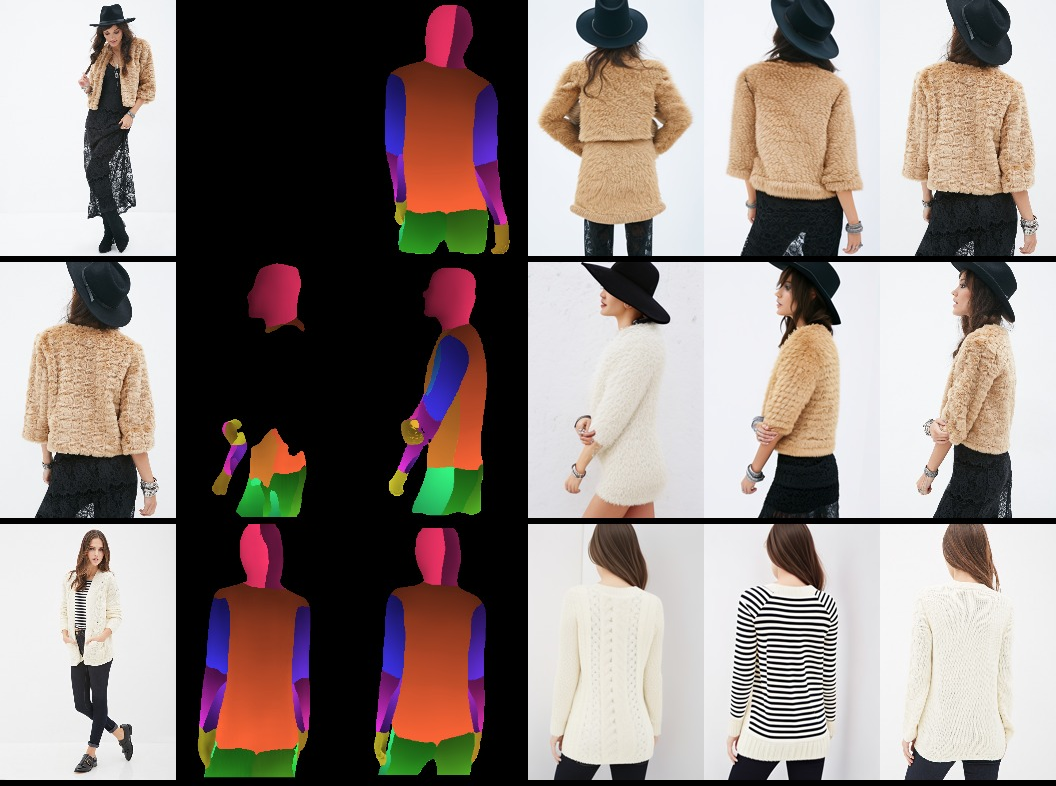
\includegraphics[width=0.86\linewidth]{figs/fig_garment.png}
\caption{\textbf{Garment transfer, rows selected \emph{by} the per-image statistics, not by eye.}
Columns: source; target-pose DensePose from detectron2 and from ours; arm~A; arm~B; ground truth.
Rows: the two largest per-image LPIPS gains and --- for honesty --- the
single worst regression in the test set, where our map drives the generator to unwrap the striped
inner layer instead of the cream knit: the double dependence that produces the gains also
propagates our errors.}
\label{fig:garment}
\end{figure}

\paragraph{Magnitude, and its denominator.}
For scale, the largest published LPIPS step on this benchmark --- our host MCLD to FPDM,
$0.1482\!\rightarrow\!0.1445$ --- is $+0.0037$, and it \emph{cost} SSIM ($-0.0094$) and FID
($+0.63$). Our change is of the same order and does not trade one metric for another, and we stop
there rather than quote a ratio: the numerator is a paired within-host delta from one harness on
identical targets, the denominator a difference between two numbers published by two groups, and
our own reproduction of MCLD differs from its published value by $0.0015$, $40\%$ of that
yardstick. The comparison establishes not a factor but a claim about attention: the correspondence
stage is not a solved input that architecture work can take for granted.

\paragraph{Standing against Leffa, on one axis.}
Leffa~\cite{leffa2025} (CVPR'25) publishes a better LPIPS than ours ($0.114$), but through a
different harness: SqueezeNet LPIPS after a 1024-px resize, against the AlexNet LPIPS of
\cref{tab:mcld}. Rather than argue from published numbers we ran Leffa's released checkpoint
ourselves and scored it and both arms on the \emph{same} $1499$ pairs under \emph{both} harnesses.
Arm~B is ahead of Leffa on every metric on both axes (\cref{tab:leffa}) and closer to
the target on $63.2\%$ of images; so is arm~A, the plain detectron2 baseline. One gap must be stated plainly: our Leffa run does not reproduce Leffa's published
numbers ($0.0969$/$0.687$ against their $0.114$/$0.732$ --- better on LPIPS, worse on SSIM),
plausibly because of our $1499$-pair subset, our generate-then-resize save path, and
pair-construction differences, so we claim a like-for-like comparison on identical inputs, not a
reproduction of their paper. The A$\rightarrow$B delta survives the change of axis
($-0.0070$ @256), so the controlled claim does not depend on which LPIPS is used.

\begin{table}[!tb]\centering\scriptsize\renewcommand{\arraystretch}{0.94}
\setlength{\tabcolsep}{4pt}
\begin{tabular}{@{}lcccccc@{}}
\toprule
 & \multicolumn{3}{c}{VtonEval (squeeze)} & \multicolumn{3}{c}{MCLD (alex)}\\
\cmidrule(lr){2-4}\cmidrule(lr){5-7}
$256$, $n{=}1499$ & LPIPS$\downarrow$ & SSIM$\uparrow$ & PSNR$\uparrow$ & LPIPS$\downarrow$ & SSIM$\uparrow$ & PSNR$\uparrow$\\
\midrule
Leffa (we ran it)  & 0.0969 & 0.6870 & 16.858 & 0.1554 & 0.6845 & 17.452\\
Arm A (detectron2) & 0.0958 & 0.7470 & 17.916 & 0.1494 & 0.7464 & 18.704\\
\textbf{Arm B (ours)} & \textbf{0.0889} & \textbf{0.7580} & \textbf{18.474} & \textbf{0.1379} & \textbf{0.7575} & \textbf{19.299}\\
\bottomrule
\end{tabular}
\caption{Leffa and both MCLD arms on identical pairs under both metric harnesses. Arm~B leads on
every metric on both axes and is closer to the target on $63.2\%$ of images; so does arm~A. Our
Leffa run does \emph{not} reproduce Leffa's published $0.114$/$0.732$ (we measure $0.0969$/$0.687$,
better on LPIPS and worse on SSIM), plausibly because of the $1499$-pair subset, our
generate-then-resize save path and pair construction, so this is a like-for-like comparison on
identical inputs, not a reproduction of their paper.}
\label{tab:leffa}
\end{table}

\section{Limitations}
\label{sec:limitations}

Every model here is a single training run, so we have no seed-to-seed variance and several
differences we report are below what we can resolve: the $0.3$-point margin of \cref{tab:coco},
smaller than the $0.4$-point spread between neighbouring checkpoints of one run; the $0.008$ spread
among the CSC gather variants; the $0.1$--$0.2^\circ$ range of the end-to-end geodesic numbers. We
have avoided ``free'' and ``noise'' for that reason, and the reported checkpoint is in addition the
maximum of a sweep evaluated on the set it is reported on. No published DensePose model has been
re-scored under our harness, so \cref{tab:coco} compares us only to ourselves. The ablations are
also narrower than the contribution list: the chart repair's AP effect is confounded with schedule
in the only near-matched comparison we ran and it is fold-free on hands and feet only; the CSC and
chart ablations are fine-tunes from a checkpoint trained at the learning rate \cref{tab:recipe}
identifies as broken, so the shipped model contains no CSC on/off comparison; and the
hidden-geometry mask and the no-resampling rule rest on label-corruption statistics rather than on
models trained with and without them --- documented requirements, not ablated components.

The frame field is supervised only by synthetic ground truth, because no real-image benchmark for
per-pixel surface orientation exists, so our real-image evidence for $\hat R$ is qualitative and it
has no baseline of any kind --- in particular not the frame obtainable by differentiating the
predicted $UV$ map. Its target is the SMPL-X \emph{body} surface, so on loose garments and hair
$\hat R$ describes a surface that is not the one seen. Horizontal flip is disabled whenever the
rotation head is active, the normal pin of \cref{eq:kabsch} is soft with a residual we never
measured, the fraction of foreground passing \cref{eq:valid} is likewise unmeasured, and we report
no GPU-hours and no inference latency. The joint COCO fine-tune buys real-domain accuracy
($0.621\!\rightarrow\!0.741$ AP) and costs held-out occlusion accuracy
($6.89^\circ\!\rightarrow\!8.24^\circ$), so we release two checkpoints rather than claim one is
best at both. Downstream, the study covers a single generator on a single domain with one training
run per arm, the swapped variable is a correspondence \emph{model} carrying its own detector and
box geometry rather than correspondence quality as a scalar, and the host consumes only $IUV$; our
Leffa comparison is like-for-like on identical inputs but on a $1499$-pair subset and does not
reproduce Leffa's published numbers.

\section{Conclusion}
\label{sec:conclusion}

We revisited the correspondence stage of DensePose --- the part of the pipeline its consumers
import and freeze --- and gave it an output it never had: a full per-pixel $SO(3)$ surface frame,
predicted alongside $IUV$. Predicting that frame correctly is what forced the rest: re-flattening
the hand and foot charts, supervising correspondence in metric template coordinates, never
resampling the labels, and training on occlusion under a sequence-level holdout. The model reaches
$0.741$ GPS AP on DensePose-COCO minival under a ground-truth-box protocol, above every model in
our own lineage while carrying the frame field --- parity with an extra output rather than a win
--- and in a controlled retrain of a CVPR'25 generator it is worth $+0.0116$ paired LPIPS, of the
same order as the largest published LPIPS step on that benchmark and without its trade-offs. Which
correspondence model a system uses is, in short, still a live variable in systems that treat it as
settled. We will release code, the two checkpoints, the \textsc{v2} chart asset and the
\textsc{v2}$\rightarrow$\textsc{v1} remap table, so the label fix can be adopted independently of
our model.



{
    \small
    \bibliographystyle{ieeenat_fullname}
    \bibliography{main}
}

\clearpage
\appendix
\setcounter{figure}{0}
\setcounter{table}{0}
\renewcommand{\thefigure}{S\arabic{figure}}
\renewcommand{\thetable}{S\arabic{table}}

\section*{Supplementary material}

This appendix carries the implementation detail removed from the main paper. It adds no result and
changes no claim; every number below is a property of an asset or an operator, not of a trained
model.

\section{The CSC operator}
\label{sup:csc}

\paragraph{Baking $T_i$.}
For each part $i$ and each texel centre $q=((a{+}\tfrac12)/K,(b{+}\tfrac12)/K)$ we find the first
chart triangle containing $q$ among the $32$ nearest chart-triangle centroids (KD-tree), take its
2D barycentrics $\beta$, and set $T_i[b,a]=\sum_k\beta_kX_k$ over the face's three template
vertices. Texels covered by no triangle are filled by clipped-barycentric projection onto the
nearest candidate, so the texture is finite and smooth everywhere and never reads garbage. Texels
claimed by more than one triangle, or by none, are flagged ambiguous and the flag is dilated by one
texel because the bilinear stencil is $2{\times}2$.

\paragraph{The read.}
$\Phi(i,u,v)$ is one 3D \texttt{grid\_sample} into a $(1,3,24,K,K)$ volume at
$\xi=2u-1$, $\eta=2v-1$, $\zeta=(2i-1)/24-1$ with \texttt{align\_corners=False}; $\zeta$ lands
exactly on the centre of slice $i{-}1$, so interpolation along the part axis is a no-op and part
selection is exact. $\Phi$ must run in \texttt{fp32}: under \texttt{bf16} autocast a $u\in[0,1]$
resolves to about one texel and the gradient signal is destroyed, so the operator disables autocast
for itself.

\paragraph{Validation gates ($K{=}512$, \textsc{v2} charts).}
(G1) Round-trip against exact barycentric XYZ on $200$k random surface points: on the $74.5\%$ of
samples the ambiguity mask admits, median $<0.001$\,mm, p99 $0.335$\,mm, \emph{max} $63.35$\,mm ---
our own pass criterion is $\max<1$\,mm, so this gate fails on its own terms and we report it as a
thin tail on sliver triangles and texel boundaries rather than as a pass. Per region, hands are
$84.5\%$ usable, feet $88.1\%$, head only $52.3\%$ --- the last is the hidden-geometry mask of
\cref{sec:data} doing its job. (G2) Autograd $\partial\Phi/\partial(u,v)$ against float64 central
differences ($h{=}10^{-7}$): median relative error $5.21\times10^{-10}$. (G3) Ground-truth $uv$
pushed through the losses: $\mathcal{L}_{\mathrm{xyz}}=0.0135$\,mm,
$\mathcal{L}_{\mathrm{grad}}=0.0056$\,mm.

\section{Orientation recipe ladder}
\label{sup:ladder}

\begin{table}[h]
\setlength{\tabcolsep}{4pt}
\centering\footnotesize
\begin{tabular}{@{}lcccc@{}}
\toprule
Configuration & geo$^\circ$ & $\Delta$ & part acc & uv $L_1$ \\
\midrule
single $6$D head, flat LR      & 9.01 & --- & 0.9621 & 0.0263 \\
$+$ per-part rotation head     & 8.48 & $-0.53$ & 0.9611 & 0.0266 \\
\quad alt.\ $+$ LLRD, $3\mathrm{e}{-}4$ \emph{(shipped)} & 8.05 & $-0.43$ & 0.9619 & 0.0259 \\
\quad alt.\ $+$ LLRD, $1\mathrm{e}{-}3$ & 7.86 & $-0.62$ & 0.9659 & 0.0251 \\
$+$ 58k$\rightarrow$120k \emph{($1\mathrm{e}{-}3$ branch)} & 7.30 & $-0.56$ & 0.9692 & 0.0228 \\
\bottomrule
\end{tabular}
\caption{Matched step 58k, \textbf{oracle} gather: the rotation channel is taken at the
ground-truth part, which measures the head in isolation and is optimistic --- on the one lineage
where we measured both, by $0.65^\circ$ ($7.30^\circ$ oracle against $7.95^\circ$ end-to-end). It
is therefore \emph{not} comparable with the deployment numbers in the main paper, a different
readout of a different lineage. ``part acc'' is $24$-way part accuracy, ``uv $L_1$'' mean
chart-unit error, both on foreground. The two LLRD rows are \emph{alternatives}, each measured
against the row above, so $\Delta$ does not telescope, and the last rung continues the branch we do
\emph{not} ship. No external baseline; single run per row.}
\label{tab:orient}
\end{table}

\begin{figure}[h]
\centering
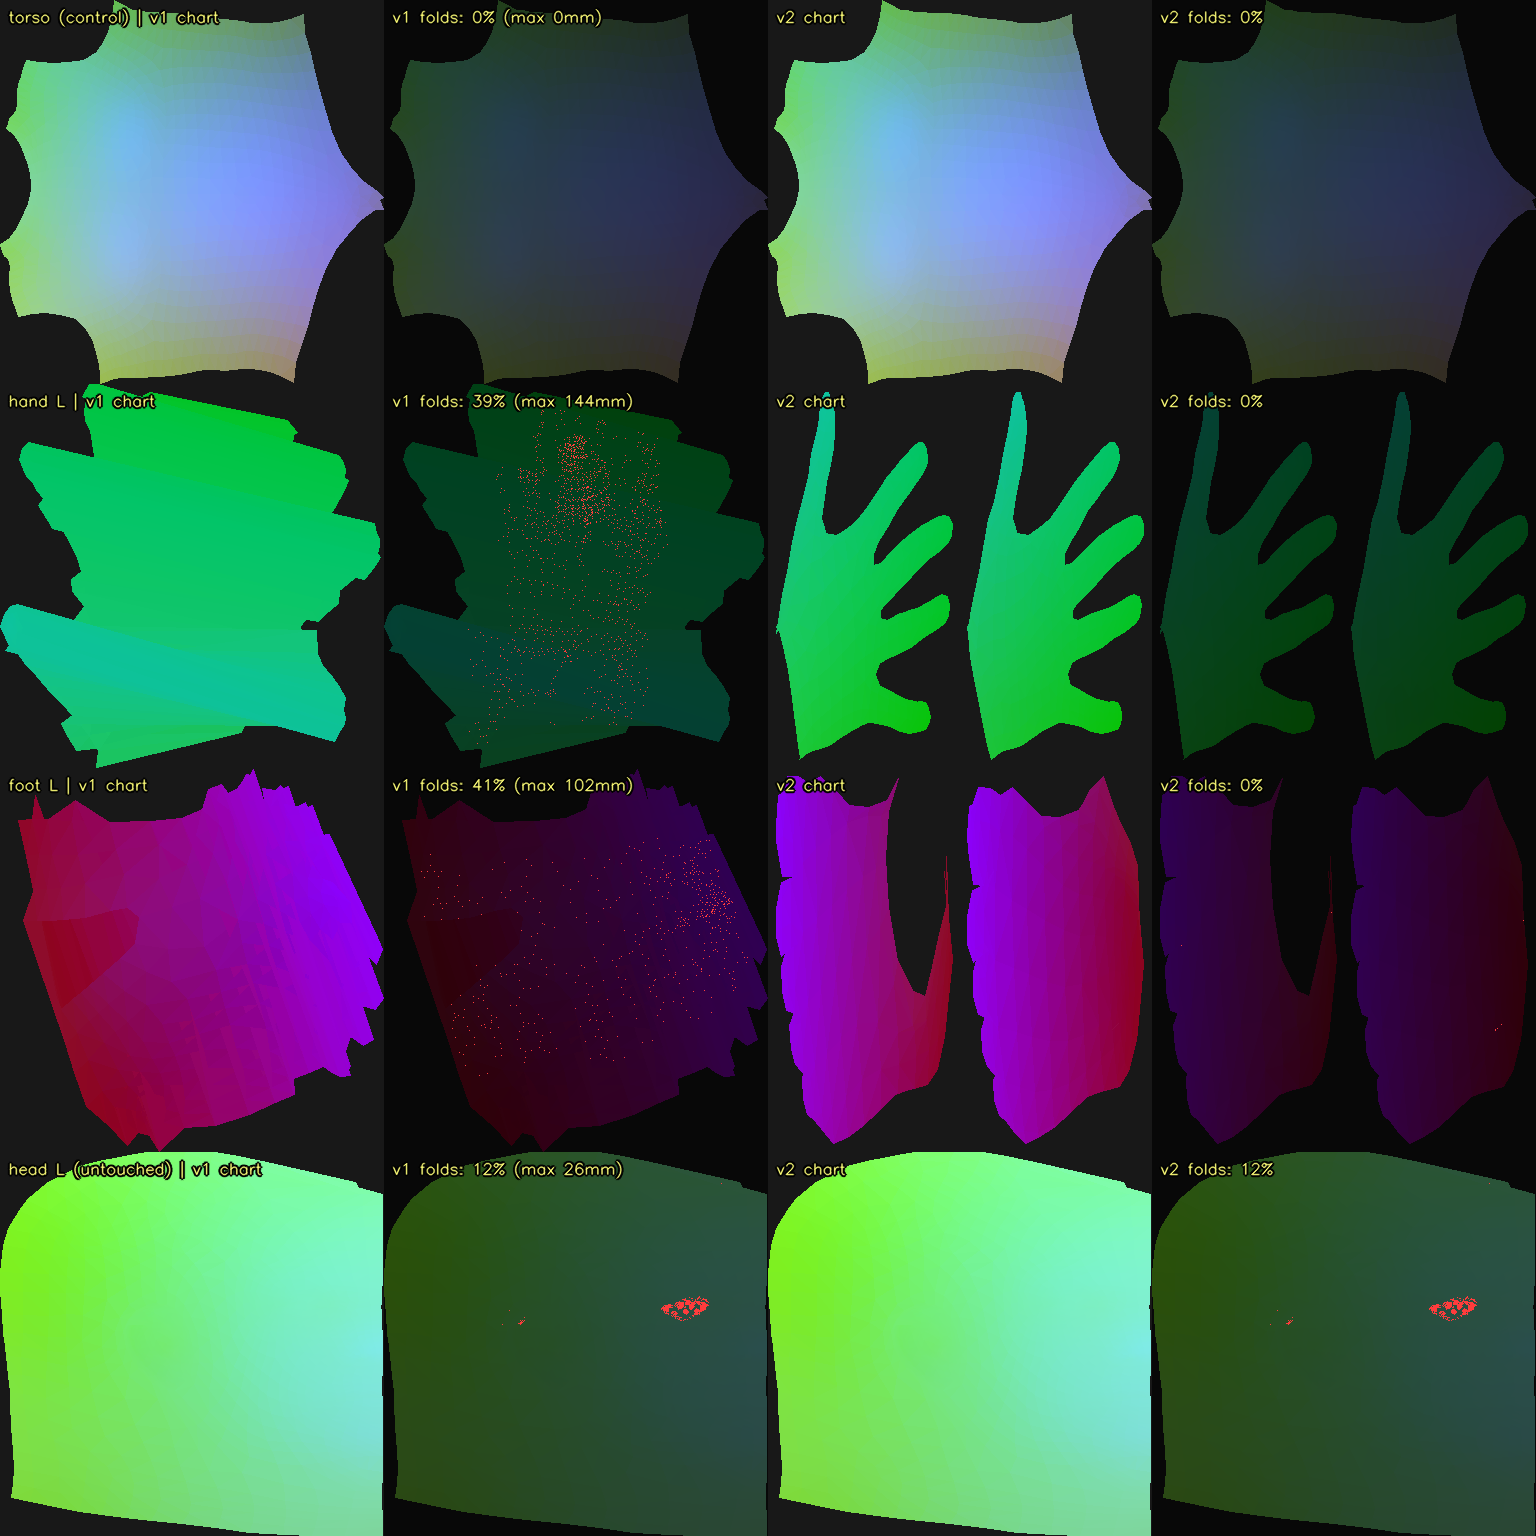
\includegraphics[width=\linewidth]{figs/fig_charts.png}
\caption{\textbf{The official DP24 atlas is non-injective on hands and feet.} Rows: torso
(control), hand, foot, head half (unchanged). Columns: the \textsc{v1} chart shaded by template
position; surface samples claimed by more than one triangle, in red; the \textsc{v2} chart; its
overlay. Annotations are chart-area weighted and quote the \emph{worst} collision; the text quotes
surface-sample fractions and the median.}
\label{fig:charts}
\end{figure}

\section{Chart re-flattening: rejected alternatives}
\label{sup:charts}

Tutte/Floater mean-value embedding gives a \emph{guaranteed} fold-free chart (exactly $0\%$ on
feet) but crushes the extremities: $409$ of $1538$ hand triangles collapse below $10^{-9}$ chart
area --- injective in exact arithmetic, degenerate in float64 --- and the texture round-trip
degrades to a median of $0.203$\,mm against $0.010$\,mm for the sheet split, i.e.\ the chart loses
resolution exactly where the artifacts were. LSCM folds outright ($122$ flipped triangles). On the
head, a spherical parameterisation is worse than the original ($69\%$ overlap) and the sheet split
reaches $32\%$; the residual there is dominated by geometry hidden \emph{inside} the part rather
than by the flattening, which is why the head is masked rather than re-cut.

\section{The fixed ground-truth canvas}
\label{sup:canvas}

Both the ground-truth canvas and the model input are axis-aligned squares in source-frame pixels,
so the map from the network's output frame into the canvas is a pure scale-and-translate affine
available in closed form. With $g_{\mathrm{side}},g_{x_0},g_{y_0}$ the canvas window and
$i_{\mathrm{size}},i_{x_0},i_{y_0}$ the input window,
\begin{equation*}
  s=\frac{g_{\mathrm{side}}}{i_{\mathrm{size}}},\qquad
  t_d=\frac{2(g_{d_0}-i_{d_0})}{i_{\mathrm{size}}}+s-1 \;\; (d\in\{x,y\}),
\end{equation*}
and $\theta_{\mathrm{warp}}=[\,[s,0,t_x],[0,s,t_y]\,]$ is fed to one \texttt{affine\_grid} /
\texttt{grid\_sample} pair per head with \texttt{align\_corners=False}; the expression is
independent of the two raster resolutions. The $144$-channel rotation field is warped in
\texttt{bf16} (fp32 activations would be $4.8$\,GB at batch $32$) and upcast only after the
six-channel gather; UV is warped in \texttt{fp32} for the reason in \cref{sup:csc}. The $4\%$ margin
between the crop's $1.25\times$ lower bound and the canvas's $1.2\times$ matters: without it,
integer rounding of the crop window left a ring of ground-truth pixels with no image support in
$2$ of $300$ sampled instances.

\section{Hidden geometry}
\label{sup:hidden}

The hidden-face set is $2176$ eyeball faces (two closed components, exactly $1088$ per eye) plus
$1694$ interior head faces ($847$ per half), the latter found with M\"oller--Trumbore: an outward
ray from the face centroid must re-hit \emph{head} geometry within $10$\,cm. Requiring the hit to be
head geometry is what removes the under-chin-to-chest false positives. Together they are $1.01\%$ of
head pixels and $0.106\%$ of foreground.

\section{Occlusion holdout}
\label{sup:holdout}

$\mathrm{md5}(\text{seq})\bmod 50=0$ selects $29$ of $2211$ sequences and $59$ of $5417$ shards
($1.1\%$), spanning all four MAMMA sub-datasets (harmony4d $3$, inter-x $20$, interactions $5$,
latindance10 $1$). Shard names embed sequence ids, so the exclusion is exact and there is no
temporal leakage between train and probe.

\section{Leffa cross-evaluation}
\label{sup:leffa}

Leffa's published numbers come from VtonEval, whose LPIPS is torchmetrics/SqueezeNet after a
1024-px resize, whereas MCLD's \texttt{evaluate.py} (and \cref{tab:mcld}) use the \texttt{lpips}
package's AlexNet LPIPS at the stated resolution; the agreement of shared baseline rows across the
two papers proves only that both copied those rows from their sources. Re-scoring our own outputs
under VtonEval's definitions gives arm~B $0.0891$/$0.1077$ LPIPS at $256$/$512$ and arm~A
$0.0961$/$0.1149$. To remove any dependence on published numbers we then ran Leffa's released
\texttt{pose\_transfer.pth} ourselves (SDXL-inpainting base, their DensePose R-50, $50$ steps,
guidance $2.5$, seed $42$) and scored Leffa and both arms on the same $1499$ pairs under both
harnesses:

\begin{figure}[h]\centering
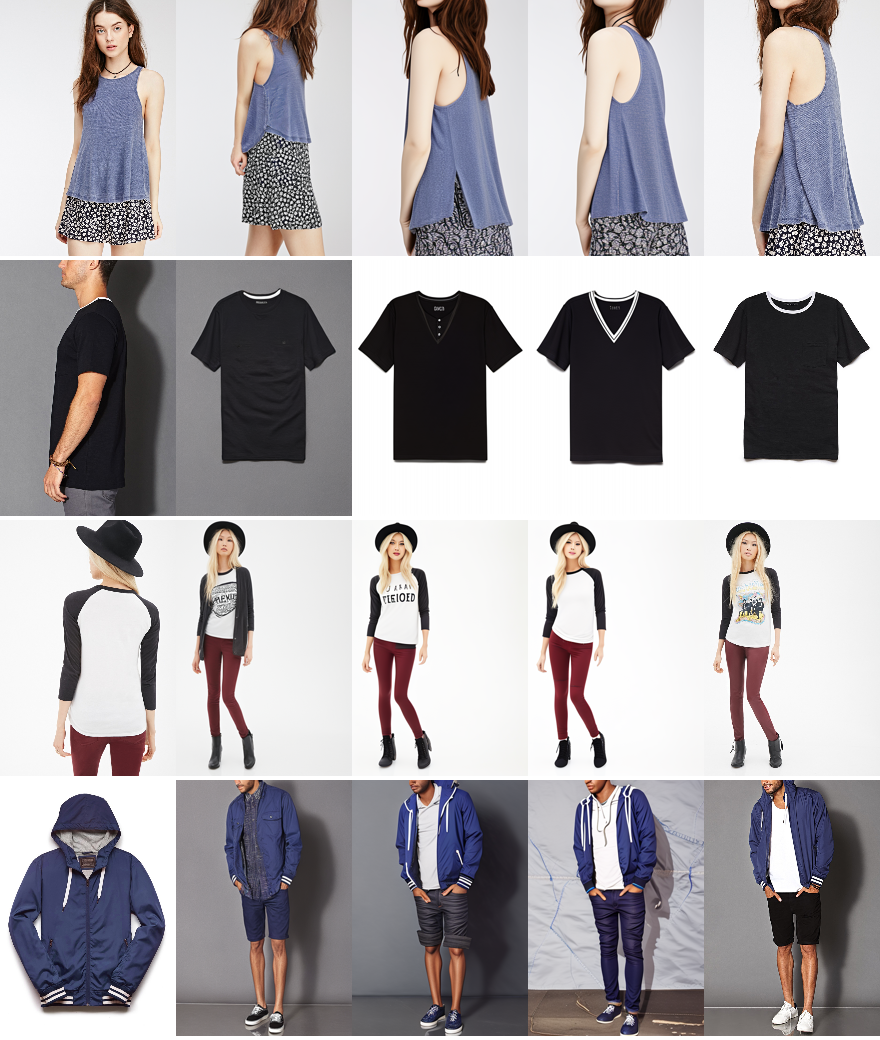
\includegraphics[width=\linewidth]{figs/fig_leffa.png}
\caption{Source, Leffa, arm~A, arm~B, ground truth. Rows are selected \emph{by} per-image LPIPS,
not curated: the two largest margins over Leffa, the median case, and the case where Leffa wins
most --- there arm~B emits a background artifact, and we include it for that reason.}
\label{fig:leffa}
\end{figure}



\end{document}
